\chapter{Omega Network}

\section{Omega Network}

Progettare e implementare in VHDL uno switch multistadio secondo il modello omega network. Lo switch deve consentire lo scambio di messaggi di 2 bit ciascuno da un nodo sorgente a un nodo destinazione in una rete con 4 nodi, implementando uno schema a priorità fissa fra i nodi (ed. nodo 1 più prioritario, con priorità decrescenti fino al nodo 4). 

\subsection{Architettura}

L'architettura è costituita da due componenti: un unità operativa e una rete di controllo.

La rete di controllo serve a gestire la priorità tra i nodi, ed è costituita da un multiplexer 4:1, un demultiplexer 1:4 ed un arbitro.
In particolare per poter inviare un dato è necessario alzare un segnale di \textit{enable}, oltre che specificare mittente, destinatario e i bit di contenuto, e l'arbitro della rete di controllo si occupa di gestire eventuale conflitti tra le abilitazioni, dando priorità in maniera statica a i primi (da 0 a 3). In questo modo si evitano possibili collisioni durante il trasferimento dei dati.
La \textit{frame} di 6 bit che entra in input attraverso le porte a0...a3 è strutturata nel seguente modo:

\begin{figure}[H]
    \centering
    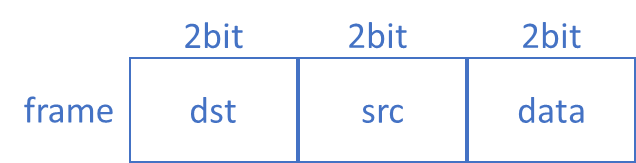
\includegraphics[width=15cm]{immagini/esercizio10/frame_omega.png}
    \caption{Frame Omega Network}
\end{figure}
Gli indirizzi di sorgente e destinazione vengono separati dai dati effettivi. I primi escono sulle omonime uscite, mentre i dati da b0...b3.

L'unità operativa implementa effettivamente il trasferimento del dato da una linea all'altra ed è costituita da un insieme di 4 switch.
Il modo in cui sono connessi questi quattro switch rispetta la definizione di omega nework che sfrutta l’idea del perfect shuffling.
Questa tecnica permette  di ottimizzare i percorsi da seguire indicando i modi di collegamento tra i diversi stadi.

\begin{figure}[H]
    \centering
    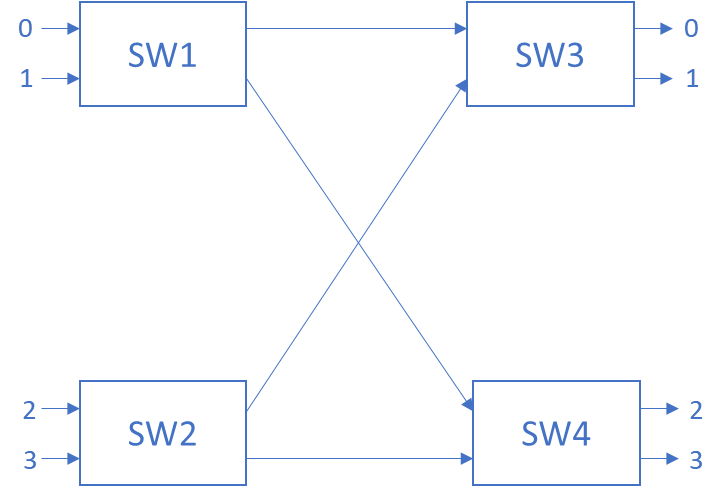
\includegraphics[width=15cm]{immagini/esercizio10/omega2x2.png}
    \caption{Frame Omega Network}
\end{figure}

Per poter determinare il percorso da seguire, una volta collegati gli switch in questa configurazione, basta leggere in ordine i bit della destinazione dal più significativo al meno significativo, e a ogni stadio usare l'uscita superiore se il bit è 0 e la inferiore se il bit è 1. Specularmente, per capire da quale sorgente leggere si leggono i bit di sorgente a partire dal meno significativo.
La comunicazione tra gli switch avviene in modalità combinatoria, e i dettagli implementativi sono mostrati nelle sezioni successive. Nel prossimo esercizio, presente tra quelli a scelta, verrà esplorata la soluzione sequenziale, che prevede un handshake tra gli switch.

\paragraph{Switch}
Lo switch è il componente fondamentale della parte operativa ed è stato progettato sulla base dell'esercizio 1.2. In particolare, è stato implementato uno \textit{switch} \textit{2x2} che collega due sorgenti a due destinazioni partendo da un \textit{multiplexer} 2:1 e un \textit{de-multiplexer} 1:2 controllati rispettivamente dai segnali di sorgente e destinazione. Nel listato\ref{switch}, è mostrata l'implementazione di uno switch. Si noti che in questa prima versione dell'esercizio, lo \textit{switch} è puramente combinatorio.


\begin{lstlisting} [language=VHDL, label=switch, caption=Switch]
library IEEE;
use IEEE.STD_LOGIC_1164.ALL;

entity switch is
  Port (
        src, dst: in std_logic;
        a0, a1: in std_logic_vector(1 downto 0);
        b0, b1: out std_logic_vector(1 downto 0)
   );
end switch;

architecture Structural of switch is

component mux_21 is
    Port (
        a0, a1: in std_logic_vector(1 downto 0);
        s : in std_logic;
        u : out std_logic_vector(1 downto 0)
    );
end component mux_21;

component demux_1_2 is
    port (
        a: in std_logic_vector(1 downto 0);
        s: in std_logic;
        u0, u1: out std_logic_vector(1 downto 0)
    );
end component demux_1_2;

signal s_link: std_logic_vector(1 downto 0);
begin

m: mux_21 port map(
    a0=>a0,
    a1=>a1,
    s => src,
    u=>s_link
);

d: demux_1_2 port map(
    a=>s_link,
    u0=>b0,
    u1 => b1,
    s=>dst
);

end Structural;
\end{lstlisting}

\paragraph{Parte operativa}
La parte operativa è stata creando istanziando 2 stadi, ciascuno composto da 2 switch. In particolare, come mostrato in Figura \ref{fig:uo_omega},al primo livello sono collegati il bit meno significativo dell'indirizzo sorgente e quello più significativo della destinazione, viceversa al secondo livello. Gli \textit{switch}, invece, sono collegati secondo la tecnica del \textit{perfect shuffling} illustrata in precedenza. I segnali di ingresso provengono dalla rete di controllo.
Infine, nel listato \ref{uo_omega}, è riportata l'implementazione con approccio strutturale dell'unità operativa.

\begin{figure}[H]
    \centering
    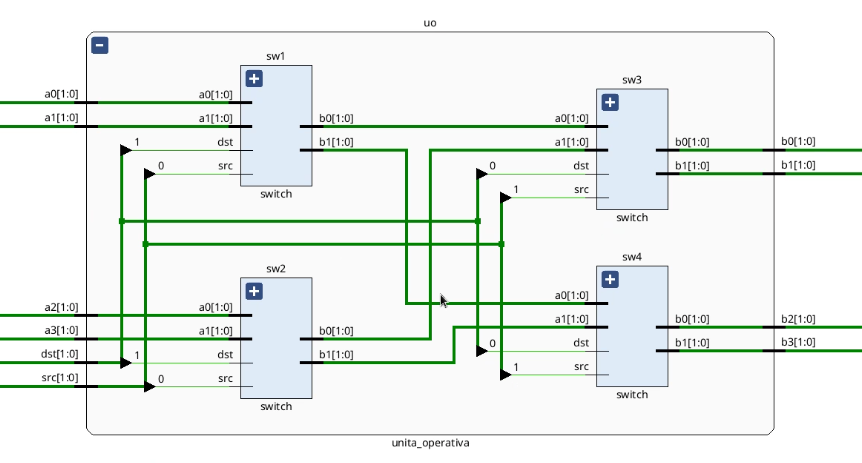
\includegraphics[width=15cm]{immagini/esercizio10/schema_10.1_unitaoperativa.png}
    \caption{Schema unità operativa omega network}
    \label{fig:uo_omega}
\end{figure}


\begin{lstlisting} [language=VHDL,label=uo_omega, caption=Unità operativa]
library IEEE;
use IEEE.STD_LOGIC_1164.ALL;

entity unita_operativa is
  Port (
        a0, a1, a2, a3: in std_logic_vector(1 downto 0);
        src, dst: in std_logic_vector(1 downto 0);
        b0, b1, b2, b3: out std_logic_vector(1 downto 0)
   );
end unita_operativa;

architecture Structural of unita_operativa is

component switch is
  Port (
        src, dst: in std_logic;
        a0, a1: in std_logic_vector(1 downto 0);
        b0, b1: out std_logic_vector(1 downto 0)
   );
end component switch;

signal s_sw1_3, s_sw1_4,  s_sw2_3, s_sw2_4 : std_logic_vector(1 downto 0);

begin
    sw1: switch port map(
        src=>src(0),
        dst=>dst(1),
        a0=> a0,
        a1=> a1,
        b0=> s_sw1_3,
        b1=> s_sw1_4
    );

    sw2: switch port map(
        src=>src(0),
        dst=>dst(1),
        a0=> a2,
        a1=> a3,
        b0=> s_sw2_3,
        b1=> s_sw2_4
    );

    sw3: switch port map(
        src=>src(1),
        dst=>dst(0),
        a0=> s_sw1_3,
        a1=> s_sw2_3,
        b0=> b0,
        b1=> b1
    );

    sw4: switch port map(
        src=>src(1),
        dst=>dst(0),
        a0=> s_sw1_4,
        a1=> s_sw2_4,
        b0=> b2,
        b1=> b3
    );

end Structural;
\end{lstlisting}

\paragraph{Rete di controllo}
La rete di controllo è un componente completamente combinatorio formato da:
\begin{itemize}
    \item multiplexer-demultiplexer: questa rete di trasmissione serve a prendere una frame completa e instradarla nell'uscita corretta dopo aver estratto gli indirizzi di sorgente e destinazione;
    \item arbitro: in questo componente arrivano i segnali di abilitazione degli utenti ($en0...en3$) che vogliono inviare una \textit{frame}. In particolare, è implementato un sistema a priorità che consente di inviare dati in mutua esclusione per evitare conflitti. Le priorità sono assegnate nel seguente modo $pr_3<pr_2<pr_1<pr_0$.
\end{itemize}

La rete di controllo mette in uscita la \textit{frame} da inviare e due segnali che corrispondono agli indirizzi sorgenti e destinazione. Questi segnali vengono dati in ingresso alla parte operativa descritta in precedenza. Infine, è riportata nel listato \ref{rc_omega} l'implementazione con approccio strutturale della rete di controllo.

\begin{lstlisting} [language=VHDL, label=rc_omega,caption=Rete di controllo]
library ieee;
use ieee.std_logic_1164.all;

entity rete_di_controllo is
    port (
        a0, a1, a2, a3: in std_logic_vector(5 downto 0);
        en0, en1, en2, en3: in std_logic;
        b0, b1, b2, b3: out std_logic_vector(1 downto 0);
        src, dst: out std_logic_vector(1 downto 0)
    );
end rete_di_controllo;

architecture Structural of rete_di_controllo is

    component arbitro is
        Port (
            en0,en1,en2,en3: in std_logic;
            u: out std_logic_vector(1 downto 0)
        );
    end component arbitro;

    component mux_4_1 is
        Port ( 
            a0,a1,a2,a3: in std_logic_vector (5 downto 0);
            s: in std_logic_vector (1 downto 0);
            u: out std_logic_vector (5 downto 0)
            );
    end component mux_4_1;

    component demux_14 is
        Port (
            a: in std_logic_vector(1 downto 0);
            s: in std_logic_vector (1 downto 0);
            u0,u1,u2,u3: out std_logic_vector(1 downto 0)
        );
    end component demux_14;

    signal s_sel: std_logic_vector(1 downto 0);
    signal s_m_out: std_logic_vector(5 downto 0);

begin
    A: arbitro port map(
            en0=>en0,
            en1=>en1,
            en2=>en2,
            en3=>en3,
            u=>s_sel
        );
    MUX: mux_4_1 port map(
            a0=>a0,
            a1=>a1,
            a2=>a2,
            a3=>a3,
            s=>s_sel,
            u => s_m_out
        );
    DEMUX: demux_14 port map(
            a=>s_m_out (1 downto 0),
            u0=>b0,
            u1=>b1,
            u2=>b2,
            u3=>b3,
            s=>s_sel
        );
    dst <= s_m_out(5 downto 4);
    src <= s_m_out(3 downto 2);

end Structural;
\end{lstlisting}


\begin{lstlisting} [language=VHDL, caption=arbitro]
library ieee;
use ieee.std_logic_1164.all;

entity arbitro is
    Port (
        en0,en1,en2,en3: in std_logic;
        u: out std_logic_vector(1 downto 0)
    );
end arbitro;

architecture Behavioral of arbitro is

begin
    u <= "00" when en0 = '1' else
         "01" when en1 = '1' else
         "10" when en2 = '1' else
         "11" when en3 = '1' else
         "00";
end Behavioral;
\end{lstlisting}


Di seguito, per completezza è riportata la \textit{omega network} implementata creando l'unità operativa e quella di controllo collegandole opportunamente tra loro.
\begin{lstlisting} [language=VHDL, caption=Omega network 2x2]
library IEEE;
use IEEE.STD_LOGIC_1164.ALL;

entity omega_network is
    Port (
        a0,a1,a2,a3: in std_logic_vector (5 downto 0);
        en0, en1, en2, en3: in std_logic;
        b0,b1,b2,b3: out std_logic_vector (1 downto 0)
    );
end omega_network;

architecture Structural of omega_network is

    component unita_operativa is
        Port (
            a0, a1, a2, a3: in std_logic_vector(1 downto 0);
            src, dst: in std_logic_vector(1 downto 0);
            b0, b1, b2, b3: out std_logic_vector(1 downto 0)
        );
    end component unita_operativa;

    component rete_di_controllo is
        port (
            a0, a1, a2, a3: in std_logic_vector(5 downto 0);
            en0, en1, en2, en3: in std_logic;
            b0, b1, b2, b3: out std_logic_vector(1 downto 0);
            src, dst: out std_logic_vector(1 downto 0)
        );
    end  component rete_di_controllo;

    signal  s_c0, s_c1, s_c2,  s_c3:  std_logic_vector(1 downto 0);
    signal s_src, s_dst :  std_logic_vector(1 downto 0);

begin
    rc: rete_di_controllo port map(
            a0 => a0,
            a1=> a1,
            a2=> a2,
            a3=> a3,
            en0=>en0,
            en1=>en1,
            en2=>en2,
            en3=>en3,
            b0=>s_c0,
            b1=> s_c1,
            b2=>s_c2,
            b3=>s_c3,
            src=>s_src,
            dst=>s_dst
        );
    uo: unita_operativa port map(
            a0 => s_c0,
            a1=> s_c1,
            a2=> s_c2,
            a3=> s_c3,
            src=>s_src,
            dst=>s_dst,
            b0=>b0,
            b1=> b1,
            b2=>b2,
            b3=>b3
        );

end Structural;
\end{lstlisting}

\subsection{Testing}
Per dimostrare il corretto funzionamento dell'intera \textit{omega network} è stata testata prima la rete di controllo (i cui risultati sono mostrati in Figura \ref{fig:sim_rc}) sottoponendola al \textit{testbench} nel listato \ref{tb_rc_omega}.

\begin{lstlisting} [language=VHDL, label=tb_rc_omega,caption=Testbench rete di controllo]
library IEEE;
use IEEE.STD_LOGIC_1164.ALL;

entity rete_di_controllo_tb is
end rete_di_controllo_tb;

architecture Behavioral of rete_di_controllo_tb is

    component rete_di_controllo is
        port (
            a0, a1, a2, a3: in std_logic_vector(5 downto 0);
            en0, en1, en2, en3: in std_logic;
            b0, b1, b2, b3: out std_logic_vector(1 downto 0);
            src, dst: out std_logic_vector(1 downto 0)
        );
    end component rete_di_controllo;

    signal s_a0, s_a1, s_a2, s_a3 :  std_logic_vector(5 downto 0) := (others => '0');
    signal s_b0, s_b1, s_b2, s_b3 :  std_logic_vector(1 downto 0) := (others => '0');
    signal s_en0, s_en1, s_en2, s_en3 :  std_logic := '0';
    signal s_src, s_dst:  std_logic_vector(1 downto 0) := (others => '0');

begin
    uut: rete_di_controllo port map (
            a0 => s_a0,
            a1=> s_a1,
            a2=> s_a2,
            a3=> s_a3,
            en0=>s_en0,
            en1=>s_en1,
            en2=>s_en2,
            en3=>s_en3,
            b0=>s_b0,
            b1=> s_b1,
            b2=>s_b2,
            b3=>s_b3,
            src=>s_src,
            dst=>s_dst
        );
            
        tb: process
            begin
                wait for 100ns;
                s_en2 <= '1';
                wait for 10 ns;
                s_a0 <= "100001";
                s_a2 <= "101001";
                wait;
        end process tb;

end Behavioral;
\end{lstlisting}

\begin{figure}[H]
    \centering
    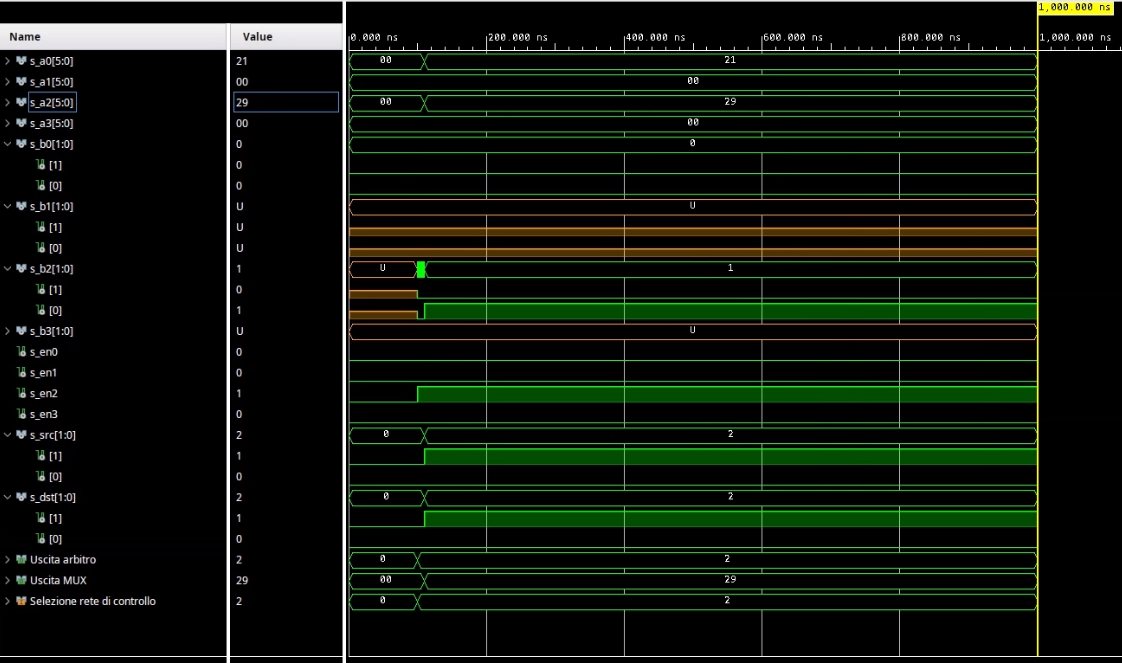
\includegraphics[width=15cm]{immagini/esercizio10/output_simulazione_10.1_retedicontrollo (da vedere se mettere).png}
    \caption{Testing rete di controllo}
    \label{fig:sim_rc}
\end{figure}

Infine, l'\textit{omega network} è stata testata provando ad inviare due \textit{frame}: la prima alzando l'abilitazione dell'utente 2, la seconda l'abilitazione dell'utente 0 (cambiando opportunamente la porta e l'indirizzo sorgente del dato). Si nota che monitorando le uscite destinatarie del pacchetto queste diventano uguali ai due bit meno significativi del \textit{frame}, come illustrato in Figura \ref{fig:sim_on}. Infine, il \textit{testbench} è illustrato nel listato che segue.

\begin{lstlisting} [language=VHDL, label=tbc_omega,caption=Testbench Omega Network]
library IEEE;
use IEEE.STD_LOGIC_1164.ALL;

entity omega_network_tb is
end omega_network_tb;

architecture Behavioral of omega_network_tb is
    component omega_network is
        Port (
            a0,a1,a2,a3: in std_logic_vector (5 downto 0);
            en0, en1, en2, en3: in std_logic;
            b0,b1,b2,b3: out std_logic_vector (1 downto 0)
        );
    end component omega_network;
    signal s_a0, s_a1, s_a2, s_a3 :  std_logic_vector(5 downto 0) := (others => '0');
    signal s_b0, s_b1, s_b2, s_b3 :  std_logic_vector(1 downto 0) := (others => '0');
    signal s_en0, s_en1, s_en2, s_en3 :  std_logic := '0';

begin
    uut: omega_network port map(
            a0 => s_a0,
            a1=> s_a1,
            a2=> s_a2,
            a3=> s_a3,
            en0=>s_en0,
            en1=>s_en1,
            en2=>s_en2,
            en3=>s_en3,
            b0=>s_b0,
            b1=> s_b1,
            b2=>s_b2,
            b3=>s_b3
        );
    process
    begin
        wait for 100ns;
        s_en2 <= '1';
        wait for 10 ns;
        s_a2 <= "101001";
        wait for 10 ns;
        assert (s_b2 = "01") report "Errore riga 44"; 
        wait for 40 ns;
        s_en0 <= '1';
        s_a0 <= "010011";
        wait for 10ns;
        assert (s_b1 = "11") report "Errore riga 48"; 
        wait;
    end process;

end Behavioral;
\end{lstlisting}


\begin{figure}[H]
    \centering
    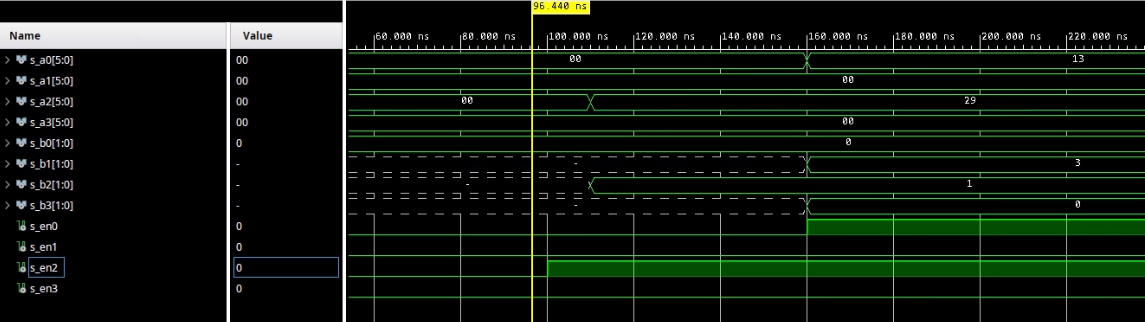
\includegraphics[width=15cm]{immagini/esercizio10/output_simulazione_10.1_omeganetwork.png}
    \caption{Testing Omega Network}
    \label{fig:sim_on}
\end{figure}

\section{Omega Network e Handshaking}
Progettare e implementare in VHDL uno switch multistadio secondo il modello omega network. 
Come punto opzionale si è scelto il punto c:
Si implementi un protocollo di handshaking semplice regolato da una coppia di segnali (pronto a inviare/pronto a ricevere) per l’invio di ciascun messaggio fra due nodi.  

\subsection{Architettura}
L'architettura di base della soluzione è simile a quella precedente. In particolare, l'introduzione della componente sincrona nei requisiti comporta una ri-progettazione della sola parte operativa (\textit{switch}) che deve essere consapevole dei dati trasmessi e ricevuti. Questa funzionalità è stata implementata aggiungendo negli \textit{switch} una rete di controllo implementata con automa a stati finiti.
Per permettere agli \textit{switch} di comunicare tramite un \textit{two-way handshake} è stata inserita al loro interno una piccola unità di controllo che si occupa di gestire i segnali di \textit{ack} e \textit{ready}. L'automa è lo stesso all'interno di tutti gli \textit{switch}, per cui è possibile istanziarne un numero a scelta senza dover effettuare modifiche. Questo rende la soluzione altamente scalabile e più facilmente testabile.
Proprio perché la comunicazione con lo \textit{switch} avviene con un \textit{handshake} sia in entrata che in uscita, anche gli utenti esterni dovranno rispettare il protocollo inviando i segnali di \textit{ack} e \textit{ready} opportunamente, quindi abbiamo un leggero aumento della grandezza della frame. 

Di seguito è mostrato l'automa della rete di controllo dello \textit{switch}:
\begin{figure}[H]
    \centering
    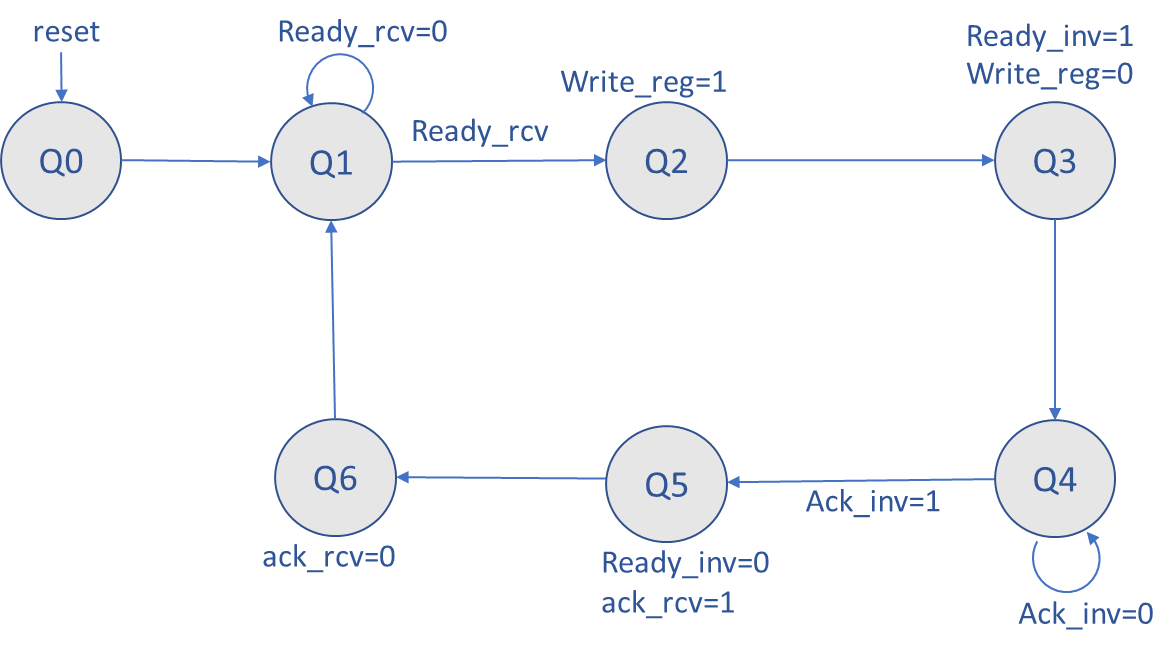
\includegraphics[width=17cm]{immagini/esercizio10/automa_10.3.png}
    \caption{Automa dello \textit{switch}}
    \label{fig:sim_rc}
\end{figure}

Come negli esercizi precedenti si aspettano i segnali di \textit{ready} e \textit{ack} per sincronizzare la comunicazione, ma invece di avere due automi separati ogni automa ha il compito di ricevere e inviare. Questo ha comportato il raddoppio dei segnali di \textit{ack} e \textit{ready}, infatti ci saranno quelli adibiti alla comunicazione con lo stadio precedente e quelli per lo stadio successivo. È stato inoltre aggiunto un semplice registro in uscita allo \textit{switch} poiché il dato non deve cambiare fino a che non arriva l'ack del destinatario.

Per semplicità negli schemi precedenti è stato mostrato l'automa e i segnali relativi a una sola uscita dello \textit{switch}, ma visto che ci sono due ingressi e due uscite tutti i segnali saranno raddoppiati, come mostrato nel seguente schema dell'architettura.

\begin{figure}[H]
    \centering
    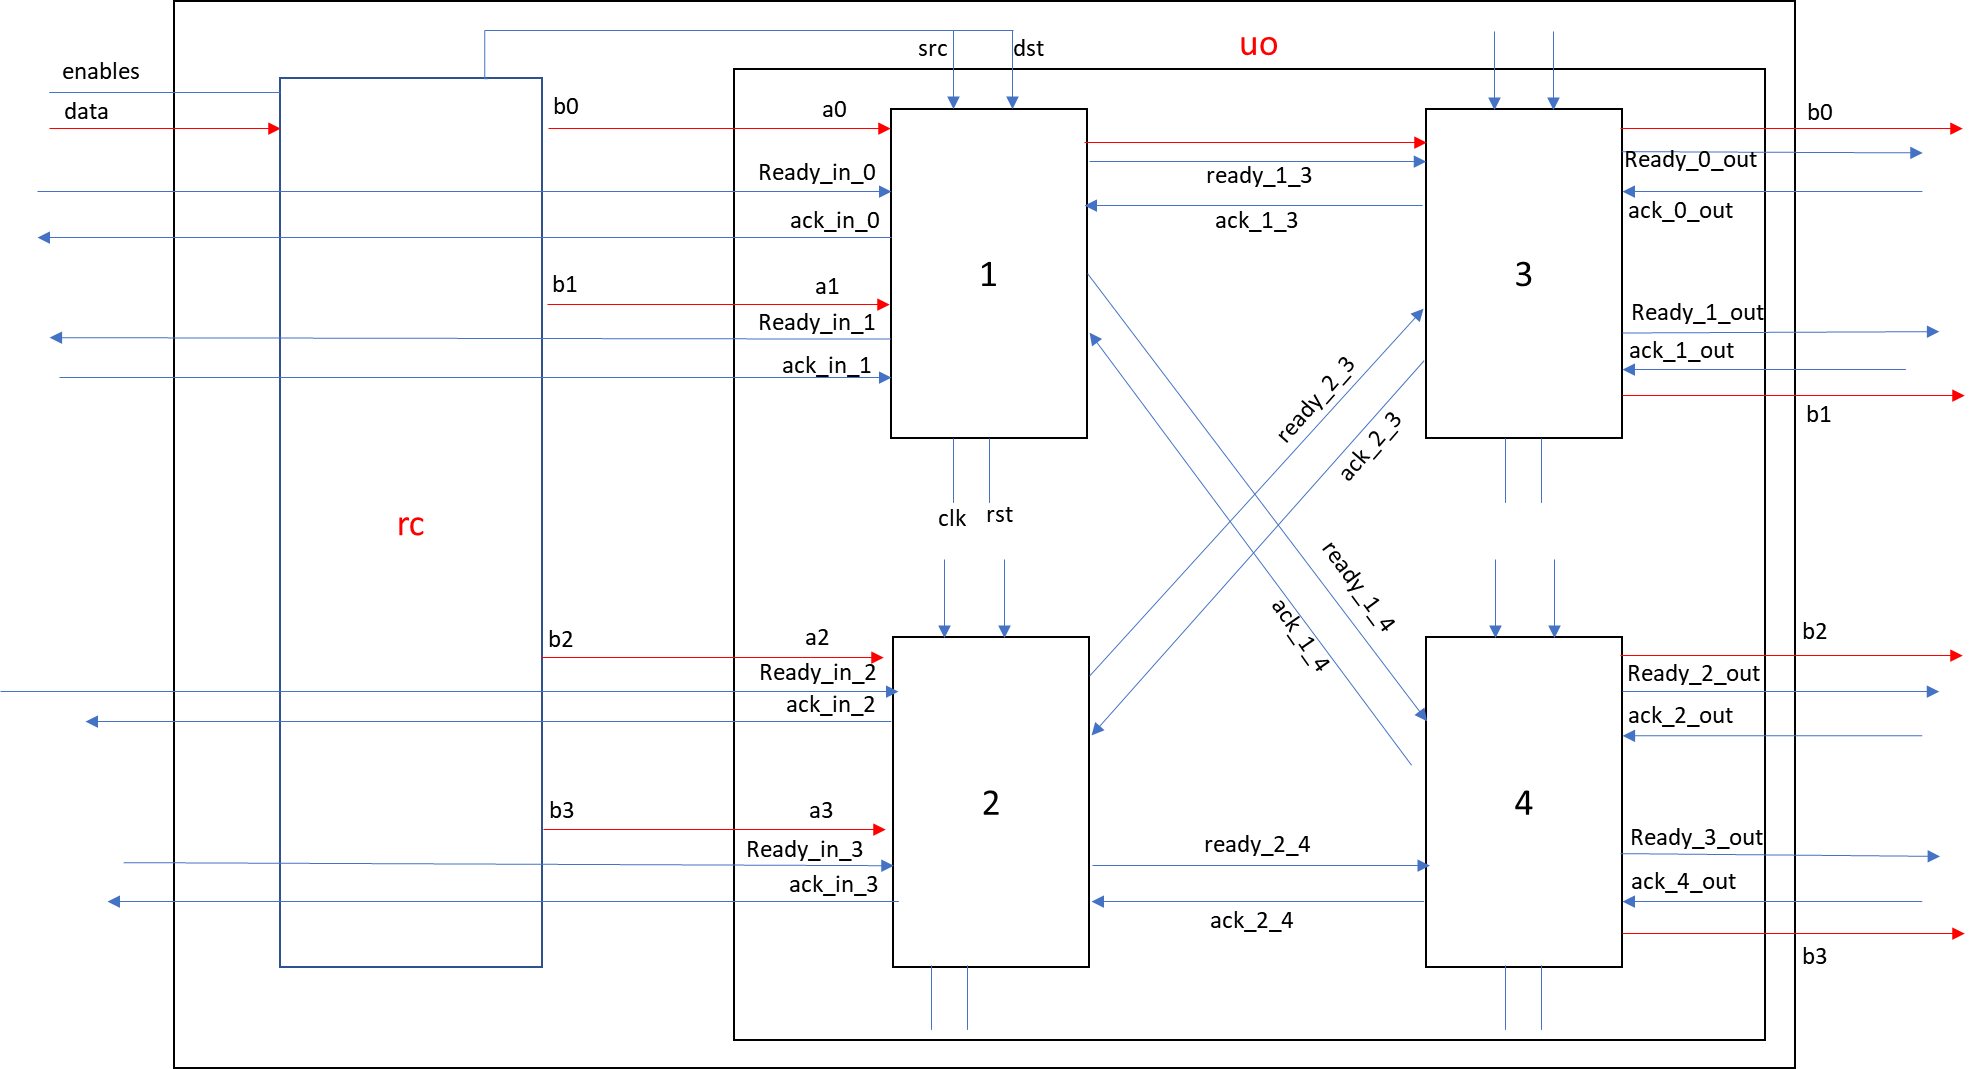
\includegraphics[width=15cm]{immagini/esercizio10/arch_tot_10.3.png}
    \caption{Architettura totale 10.3}
    \label{fig:sim_rc}
\end{figure}

\begin{lstlisting} [language=VHDL, caption=Rete di controllo switch]
library IEEE;
use IEEE.STD_LOGIC_1164.ALL;
use ieee.numeric_std.all;

entity rc_switch is
    port(
        clk, reset, ack0_snd, ready0_rcv, ack1_snd, ready1_rcv, dst, src: in std_logic;
        ack0_rcv, ready0_snd, ack1_rcv, ready1_snd,write_reg0, write_reg1: out std_logic
    );
end rc_switch;

architecture behavioral of rc_switch is
    type stato is (Q0, Q1, Q2, Q3, Q4, Q5, Q6);
    signal stato_corrente : stato:= Q0;
    signal stato_prossimo : stato;

begin
    comb: process(stato_corrente, ack0_snd, ready0_rcv, ack1_snd, ready1_rcv)

    begin
        case stato_corrente is
            when Q0=>
                stato_prossimo<=Q1;
                ready0_snd <= '0';
                ack0_rcv <= '0';
                ready1_snd <= '0';
                ack1_rcv <= '0';
                write_reg0<= '0';
                write_reg1<= '0';

            when Q1=>
                if (src = '0') then
                    if(ready0_rcv='1') then
                        stato_prossimo<=Q2;
                    else
                        stato_prossimo<=Q1;
                    end if;
                elsif (src ='1')  then
                    if(ready1_rcv='1') then
                        stato_prossimo<=Q2;
                    else
                        stato_prossimo<=Q1;
                    end if;
                end if;

            when Q2=>
                write_reg0<='1';
                write_reg1<= '1';
                stato_prossimo<=Q3;

            when Q3=>
                write_reg0<= '0';
                write_reg1<= '0';
                
                if (dst = '0') then
                    ready0_snd <= '1';
                elsif (dst ='1')  then
                    ready1_snd <= '1';
                end if;
                
                stato_prossimo<=Q4;

            when Q4=>
                 if (dst = '0') then
                    if(ack0_snd='1') then
                        stato_prossimo<=Q5;
                    else
                        stato_prossimo<=Q4;
                    end if;
                elsif (dst ='1')  then
                    if(ack1_snd='1') then
                        stato_prossimo<=Q5;
                    else
                        stato_prossimo<=Q4;
                    end if;
                end if;

            when Q5=>
                if (dst='0') then
                    ready0_snd <= '0';
                    elsif (dst='1') then
                        ready1_snd <= '0';
                end if;
                
                if (src='0') then
                    ack0_rcv <= '1';
                elsif (src='1') then
                    ack1_rcv <= '1';
                end if;
 
                stato_prossimo <=Q6;

            when Q6=>
                ack0_rcv<='0';
                ack1_rcv <= '0';
                stato_prossimo <=Q1;
            when others => stato_prossimo<= Q0;
        end case;
    end process comb;

    seq: process(clk)
    begin
        if rising_edge(clk) then
            if(reset='1')then
                stato_corrente<=Q0;
            else
                stato_corrente<=stato_prossimo;
            end if;
        end if;
    end process seq;
end behavioral;
\end{lstlisting}


Al contrario dell'esercizio precedente, questo \textit{switch} è una macchina sequenziale la cui implementazione è riportata nel listato di seguito.
\begin{lstlisting} [language=VHDL, caption=Switch sincrono]
library IEEE;
use IEEE.STD_LOGIC_1164.ALL;

entity switch is
    Port (
        src, dst, rst, clk, ack0_snd,ack1_snd, ready0_rcv,ready1_rcv: in std_logic;
        a0, a1: in std_logic_vector(1 downto 0);
        b0, b1: out std_logic_vector(1 downto 0);
        ack0_rcv, ack1_rcv, ready0_snd,ready1_snd: out std_logic
    );
end switch;

architecture Structural of switch is
    component mux_21 is
        Port (
            a0, a1: in std_logic_vector(1 downto 0);
            s : in std_logic;
            u : out std_logic_vector(1 downto 0)
        );
    end component mux_21;

    component demux_1_2 is
        port (
            a: in std_logic_vector(1 downto 0);
            s: in std_logic;
            u0, u1: out std_logic_vector(1 downto 0)
        );
    end component demux_1_2;

    component rc_switch is
        port(
            clk, reset, ack0_snd, ready0_rcv, ack1_snd, ready1_rcv, dst, src: in std_logic;
            ack0_rcv, ready0_snd, ack1_rcv, ready1_snd,write_reg0, write_reg1: out std_logic
        );
    end component rc_switch;

    component flip_flop is
        port (
            d: in std_logic_vector (1 downto 0);
            clk, reset: in std_logic ;
            write: in std_logic ;
            q:out std_logic_vector (1 downto 0));
    end component flip_flop;

    signal s_link, s_u0, s_u1: std_logic_vector(1 downto 0);
    signal s_write0, s_write1: std_logic;
begin

    m: mux_21 port map(
            a0=>a0,
            a1=>a1,
            s => src,
            u=>s_link
        );

    d: demux_1_2 port map(
            a=>s_link,
            u0=>s_u0,
            u1 => s_u1,
            s=>dst
        );

    ff1: flip_flop port map(
            d=>s_u0,
            q=>b0,
            clk=>clk,
            reset=>rst,
            write=>s_write0
        );

    ff2: flip_flop port map(
            d=>s_u1,
            q=>b1,
            clk=>clk,
            reset=>rst,
            write=>s_write1
        );

    rc: rc_switch port map(
            clk=>clk,
            reset=>rst,
            write_reg0=> s_write0,
            write_reg1=> s_write1,
            ack0_snd=>ack0_snd,
            ack1_snd=>ack1_snd,
            ready0_snd=> ready0_snd,
            ready1_snd=> ready1_snd,
            ack0_rcv=>ack0_rcv,
            ack1_rcv=>ack1_rcv,
            ready0_rcv=>ready0_rcv,
            ready1_rcv=>ready1_rcv,
            dst=>dst,
            src=>src
        );

end Structural;

\end{lstlisting}

\begin{lstlisting} [language=VHDL, caption=Arbitro]
library IEEE;
use IEEE.STD_LOGIC_1164.ALL;

entity unita_operativa is
  Port (
        a0, a1, a2, a3: in std_logic_vector(1 downto 0);
        src, dst: in std_logic_vector(1 downto 0);
        b0, b1, b2, b3: out std_logic_vector(1 downto 0);
        rst,clk: in std_logic ;
        
        ready_in_0,ready_in_1,ready_in_2,ready_in_3: in std_logic ;
        ack_in_0,ack_in_1,ack_in_2,ack_in_3: out std_logic ;
        ready_0_out, ready_1_out,ready_2_out,ready_3_out: out std_logic ;
        ack_0_out,ack_1_out,ack_2_out, ack_3_out: in std_logic
      
   );
end unita_operativa;

architecture Structural of unita_operativa is

component switch is
    Port (
        src, dst, rst, clk, ack0_snd,ack1_snd, ready0_rcv,ready1_rcv: in std_logic;
        a0, a1: in std_logic_vector(1 downto 0);
        b0, b1: out std_logic_vector(1 downto 0);
        ack0_rcv, ack1_rcv, ready0_snd,ready1_snd: out std_logic
    );
end component switch;
--dati
signal s_sw1_3, s_sw1_4,  s_sw2_3, s_sw2_4 : std_logic_vector(1 downto 0);

--ack e ready
signal s_ack_1_3, s_ack_1_4,s_ack_2_3,s_ack_2_4, s_ready_1_3, s_ready_1_4,s_ready_2_3,s_ready_2_4: std_logic;

begin

sw1: switch port map(
    src=>src(0),
    dst=>dst(1),
    a0=> a0,
    a1=> a1,
    
    ack0_rcv=> ack_in_0,
    ack1_rcv=> ack_in_1,
    
    ready0_snd=> s_ready_1_3,
    ready1_snd=> s_ready_1_4,
    
    ack0_snd=>s_ack_1_3,
    ack1_snd=>s_ack_1_4,
  
    ready0_rcv=> ready_in_0,
    ready1_rcv=> ready_in_1,    
    
    b0=> s_sw1_3,
    b1=> s_sw1_4,
    
    rst=> rst,
    clk=>clk
);

sw2: switch port map(
    src=>src(0),
    dst=>dst(1),
    a0=> a2,
    a1=> a3,
    
    ack0_rcv=> ack_in_2,
    ack1_rcv=> ack_in_3,
    
    ready0_snd=> s_ready_2_3,
    ready1_snd=> s_ready_2_4,
    
    ack0_snd=>s_ack_2_3,
    ack1_snd=>s_ack_2_4,
  
    ready0_rcv=> ready_in_2,
    ready1_rcv=> ready_in_3,    
    
    b0=> s_sw2_3,
    b1=> s_sw2_4,
    
    rst=> rst,
    clk=>clk
);


sw3: switch port map(
    src=>src(1),
    dst=>dst(0),
    a0=> s_sw1_3,
    a1=> s_sw2_3,
    
    ack0_rcv=> s_ack_1_3 ,
    ack1_rcv=> s_ack_2_3,
    
    ready0_snd=> ready_0_out,
    ready1_snd=> ready_1_out,
    
    ack0_snd=>ack_0_out,
    ack1_snd=>ack_1_out,
  
    ready0_rcv=> s_ready_1_3,
    ready1_rcv=> s_ready_2_3,    
    
    b0=> b0,
    b1=> b1,
    
    rst=> rst,
    clk=>clk
);

sw4: switch port map(
    src=>src(1),
    dst=>dst(0),
    a0=> s_sw1_4,
    a1=> s_sw2_4,
    
    ack0_rcv=> s_ack_1_4 ,
    ack1_rcv=> s_ack_2_4,
    
    ready0_snd=> ready_2_out,
    ready1_snd=> ready_3_out,
    
    ack0_snd=>ack_2_out,
    ack1_snd=>ack_3_out,
  
    ready0_rcv=> s_ready_1_4,
    ready1_rcv=> s_ready_2_4,    
    
    b0=> b2,
    b1=> b3,
    
    rst=> rst,
    clk=>clk
);

end Structural;
\end{lstlisting}

Infine, di seguito è presentato il codice dell'omega network \textbf{sincrona}:
\begin{lstlisting} [language=VHDL, caption=Omega Network]
library IEEE;
use IEEE.STD_LOGIC_1164.ALL;

entity omega_network is
    Port (
        a0,a1,a2,a3: in std_logic_vector (5 downto 0);
        en0, en1, en2, en3, clk, rst: in std_logic;
        b0,b1,b2,b3: out std_logic_vector (1 downto 0);

        ready_in_0,ready_in_1,ready_in_2,ready_in_3: in std_logic ;
        ack_in_0,ack_in_1,ack_in_2,ack_in_3: out std_logic ;
        ready_0_out, ready_1_out,ready_2_out,ready_3_out: out std_logic ;
        ack_0_out,ack_1_out,ack_2_out, ack_3_out: in std_logic

    );
end omega_network;

architecture Structural of omega_network is

    component unita_operativa is
        Port (
            a0, a1, a2, a3: in std_logic_vector(1 downto 0);
            src, dst: in std_logic_vector(1 downto 0);
            b0, b1, b2, b3: out std_logic_vector(1 downto 0);
            rst,clk: in std_logic ;

            ready_in_0,ready_in_1,ready_in_2,ready_in_3: in std_logic ;
            ack_in_0,ack_in_1,ack_in_2,ack_in_3: out std_logic ;
            ready_0_out, ready_1_out,ready_2_out,ready_3_out: out std_logic ;
            ack_0_out,ack_1_out,ack_2_out, ack_3_out: in std_logic

        );
    end component unita_operativa;

    component rete_di_controllo is
        port (
            a0, a1, a2, a3: in std_logic_vector(5 downto 0);
            en0, en1, en2, en3: in std_logic;
            b0, b1, b2, b3: out std_logic_vector(1 downto 0);
            src, dst: out std_logic_vector(1 downto 0)
        );
    end  component rete_di_controllo;

    signal  s_c0, s_c1, s_c2,  s_c3:  std_logic_vector(1 downto 0);
    signal s_src, s_dst :  std_logic_vector(1 downto 0);

begin

    rc: rete_di_controllo port map(
            a0 => a0,
            a1=> a1,
            a2=> a2,
            a3=> a3,
            en0=>en0,
            en1=>en1,
            en2=>en2,
            en3=>en3,
            b0=>s_c0,
            b1=> s_c1,
            b2=>s_c2,
            b3=>s_c3,
            src=>s_src,
            dst=>s_dst
        );

    uo: unita_operativa port map(
            a0 => s_c0,
            a1=> s_c1,
            a2=> s_c2,
            a3=> s_c3,
            src=>s_src,
            dst=>s_dst,
            b0=>b0,
            b1=> b1,
            b2=>b2,
            b3=>b3,
            clk=> clk,
            rst=> rst,

            ready_in_0=> ready_in_0,
            ready_in_1=>ready_in_1,
            ready_in_2=>ready_in_2,
            ready_in_3=>ready_in_3,
            ack_in_0=>ack_in_0,
            ack_in_1=>ack_in_1,
            ack_in_2=>ack_in_2,
            ack_in_3=>ack_in_3,
            ready_0_out=>ready_0_out,
            ready_1_out=>ready_1_out,
            ready_2_out=>ready_2_out,
            ready_3_out=>ready_3_out,
            ack_0_out=>ack_0_out,
            ack_1_out=>ack_1_out,
            ack_2_out=>ack_2_out,
            ack_3_out=>ack_3_out
        );

end Structural;

\end{lstlisting}

\subsection{Testing}
Per una maggiore sicurezza si è scelto di testare prima la rete di controllo dello \textit{switch} singolo, poi la rete di controllo dell'intero sistema (il cui test è omesso poiché analogo a quello dell'esercizio precedente) e infine si è effettuata la simulazione dell'omega network.

Di seguito è mostrato il \textit{testbench} della rete di controllo dello \textit{switch} il cui risultato è mostrato in 
 Figura \ref{fig:sim_rc_10_3}.
\begin{lstlisting} [language=VHDL, caption= Testing della rete di controllo dello switch]
library IEEE;
use IEEE.STD_LOGIC_1164.ALL;

entity switch_rc_TB is

end switch_rc_TB;

architecture Behavioral of switch_rc_TB is

component rc_switch is
    port(
        clk, reset, ack0_snd, ready0_rcv, ack1_snd, ready1_rcv, dst, src: in std_logic;
        ack0_rcv, ready0_snd, ack1_rcv, ready1_snd,write_reg0, write_reg1: out std_logic
    );
end component rc_switch;

    signal s_clk, s_reset, s_ack0_snd, s_ready0_rcv, s_ack1_snd, s_ready1_rcv, s_dst, s_src :  std_logic := '0';
    signal s_ack0_rcv, s_ready0_snd, s_ack1_rcv, s_ready1_snd, s_write_reg0, s_write_reg1 : std_logic := '0'; 

    constant clk_period:time:= 10ns;
begin

uut: rc_switch port map(
            clk=>s_clk,
            reset=>s_reset,
            write_reg0=> s_write_reg0,
            write_reg1=> s_write_reg1,
            ack0_snd=>s_ack0_snd,
            ack1_snd=>s_ack1_snd,
            ready0_snd=> s_ready0_snd,
            ready1_snd=> s_ready1_snd,
            ack0_rcv=>s_ack0_rcv,
            ack1_rcv=>s_ack1_rcv,
            ready0_rcv=>s_ready0_rcv,
            ready1_rcv=>s_ready1_rcv,
            dst=>s_dst,
            src=>s_src
        );

clock: process
    begin
           s_clk<= '1';
            wait for clk_period/2;
           s_clk <= '0';
            wait for clk_period/2;
    end process clock;

  tb: process
            begin
                wait for 100ns;
                s_reset<='1';
                wait for 10 ns;
                s_reset<='0';
                s_src<='0';
                s_dst <='0';
                wait for 10 ns;
                
                s_ready0_rcv <='1';
                wait for 30 ns;
                s_ready0_rcv <='0';
                wait for 30 ns;
                s_ack0_snd <='1';
                wait for 10 ns;
                s_ack0_snd <='0';
                wait for 40 ns;
                
                wait;
        end process tb;

end Behavioral;

\end{lstlisting}


\begin{figure}[H]
    \centering
    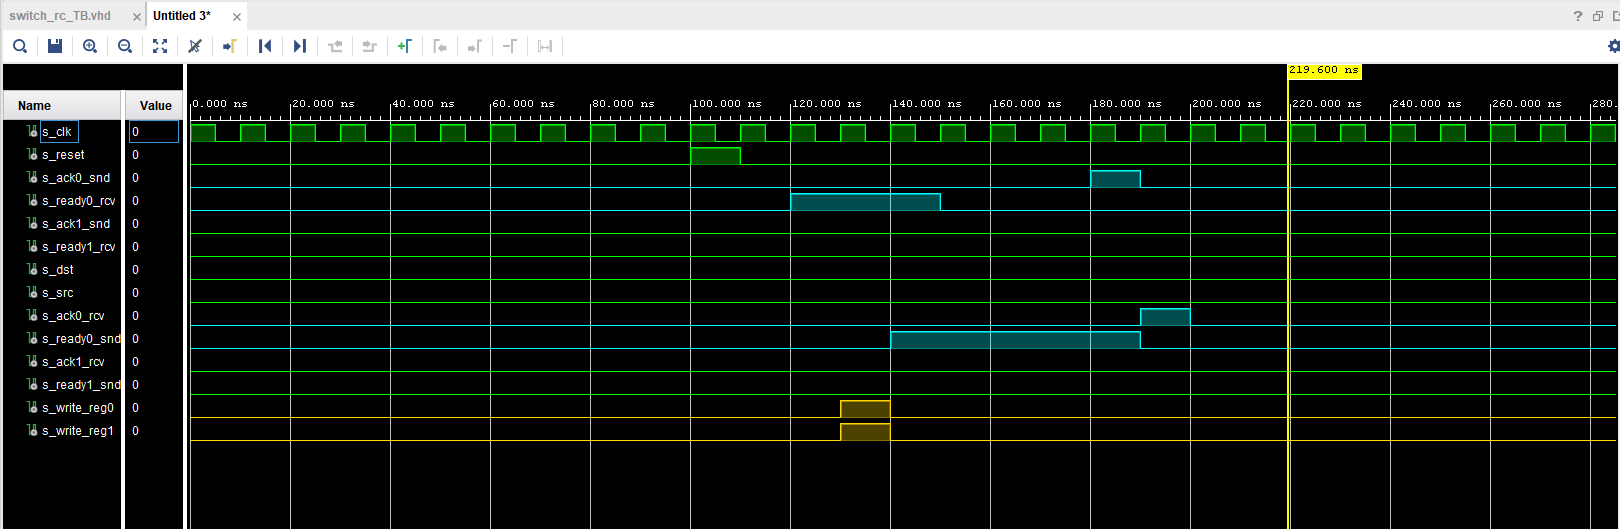
\includegraphics[width=15cm]{immagini/esercizio10/simulazione_rc_10.3.png}
    \caption{Testing rete di controllo switch}
    \label{fig:sim_rc_10_3}
\end{figure}


Infine, è presentato il \textit{testing} della \textit{omega network} sincrona con la simulazione in Figura \ref{fig:sim_on_sync}. 
\begin{lstlisting} [language=VHDL, caption=Testing dell'omega network]
library IEEE;
use IEEE.STD_LOGIC_1164.ALL;

entity omega_network_tb is
end omega_network_tb;

architecture Behavioral of omega_network_tb is

    component omega_network is
        Port (
            a0,a1,a2,a3: in std_logic_vector (5 downto 0);
            en0, en1, en2, en3, clk, rst: in std_logic;
            b0,b1,b2,b3: out std_logic_vector (1 downto 0);

            ready_in_0,ready_in_1,ready_in_2,ready_in_3: in std_logic ;
            ack_in_0,ack_in_1,ack_in_2,ack_in_3: out std_logic ;
            ready_0_out, ready_1_out,ready_2_out,ready_3_out: out std_logic ;
            ack_0_out,ack_1_out,ack_2_out, ack_3_out: in std_logic

        );
    end component omega_network;

    signal s_a0, s_a1, s_a2, s_a3 :  std_logic_vector(5 downto 0) := (others => '0');
    signal s_b0, s_b1, s_b2, s_b3 :  std_logic_vector(1 downto 0) := (others => '0');
    signal s_en0, s_en1, s_en2, s_en3, s_clk, s_rst :  std_logic := '0';
    signal s_ready_in_0,s_ready_in_1,s_ready_in_2,s_ready_in_3:  std_logic := '0';
    signal s_ack_in_0,s_ack_in_1,s_ack_in_2,s_ack_in_3:  std_logic := '0';
    signal s_ready_0_out, s_ready_1_out,s_ready_2_out,s_ready_3_out:  std_logic:= '0' ;
    signal s_ack_0_out,s_ack_1_out,s_ack_2_out, s_ack_3_out:  std_logic := '0';
    
    constant clk_period:time:= 10ns;

begin
    uut: omega_network port map(
            a0 => s_a0,
            a1=> s_a1,
            a2=> s_a2,
            a3=> s_a3,
            en0=>s_en0,
            en1=>s_en1,
            en2=>s_en2,
            en3=>s_en3,
            b0=>s_b0,
            b1=> s_b1,
            b2=>s_b2,
            b3=>s_b3,
            clk=> s_clk,
            rst=> s_rst,
            
            ready_in_0=> s_ready_in_0,
            ready_in_1=>s_ready_in_1,
            ready_in_2=>s_ready_in_2,
            ready_in_3=>s_ready_in_3,
            ack_in_0=>s_ack_in_0,
            ack_in_1=>s_ack_in_1,
            ack_in_2=>s_ack_in_2,
            ack_in_3=>s_ack_in_3,
            ready_0_out=>s_ready_0_out,
            ready_1_out=>s_ready_1_out,
            ready_2_out=>s_ready_2_out,
            ready_3_out=>s_ready_3_out,
            ack_0_out=>s_ack_0_out,
            ack_1_out=>s_ack_1_out,
            ack_2_out=>s_ack_2_out,
            ack_3_out=>s_ack_3_out
        );

    clock: process
    begin
        s_clk<= '1';
        wait for clk_period/2;
        s_clk <= '0';
        wait for clk_period/2;
    end process clock;

    process
    begin
        wait for 100ns;
        s_rst<='1';
        wait for 10 ns;
        s_rst<='0';
        wait for 10 ns;
        s_en0 <= '1';

        --dst --src  -a -r --data

        wait for 10 ns;
        s_a0 <= "010011";
        s_ready_in_0<='1';
        wait for 10 ns;
        s_ready_in_0<='0';
        wait for 10 ns;
        
        wait until s_ready_1_out='1';
        wait for 10 ns;
        s_ack_1_out<='1';
        wait for 10 ns;
        s_ack_1_out<='0';
        
        wait until s_ack_in_0='1';
        wait for 10 ns;
        
        report "received";
     wait;
    end process;

end Behavioral;

\end{lstlisting}


\begin{figure}[H]
    \centering
    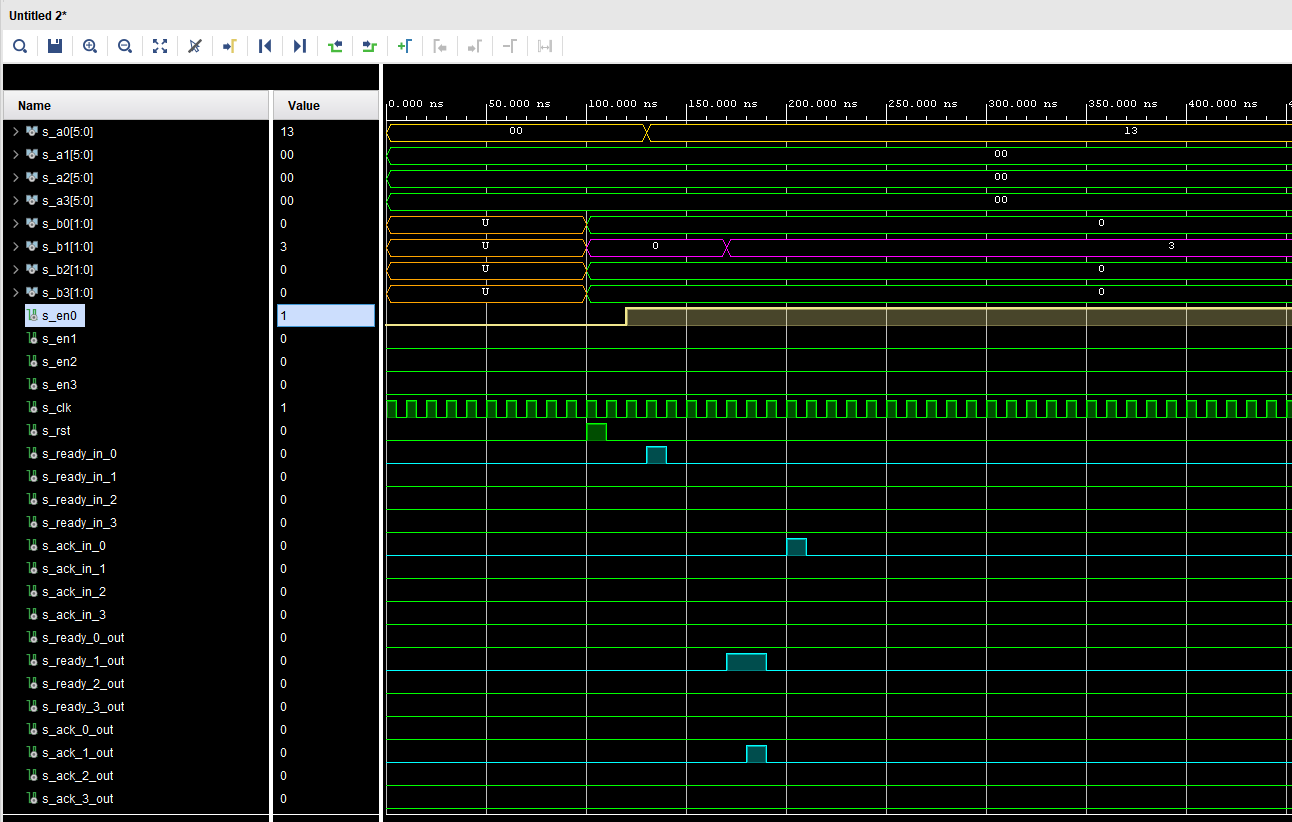
\includegraphics[width=15cm]{immagini/esercizio10/output_simulazione_10.3.png}
    \caption{Testing Omega Network sincrona}
    \label{fig:sim_on_sync}
\end{figure}
